\documentclass[a4paper, 12pt, final, garamond]{book}
\usepackage{cours-preambule}

\raggedbottom

\makeatletter
\renewcommand{\@chapapp}{Programme de kh\^olle -- semaine}
\makeatother

\begin{document}
\setcounter{chapter}{2}

\chapter{Du 26 au 30 septembre}

\begin{figure}[h]
    \vspace{-20pt}
    \centering
    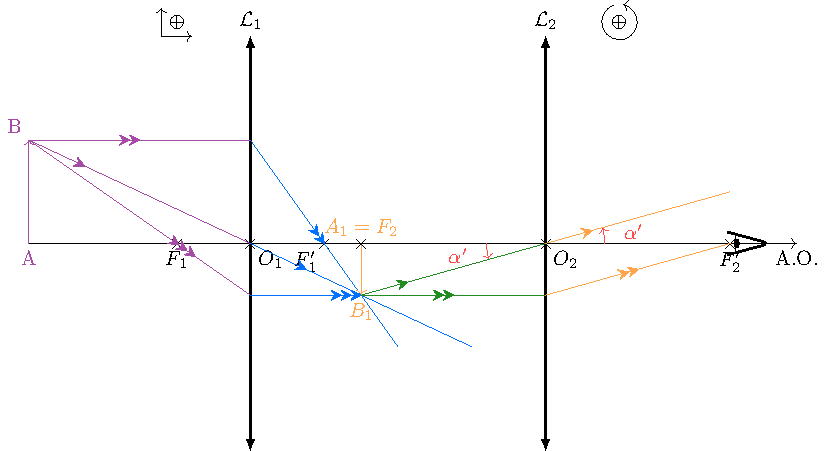
\includegraphics[width=\linewidth]{microscope}
    \captionsetup{justification=centering}
    \caption{Schéma pour le microscope.}
    \label{fig:micro}
\end{figure}
\begin{figure}[h]
    \vspace{-20pt}
    \centering
    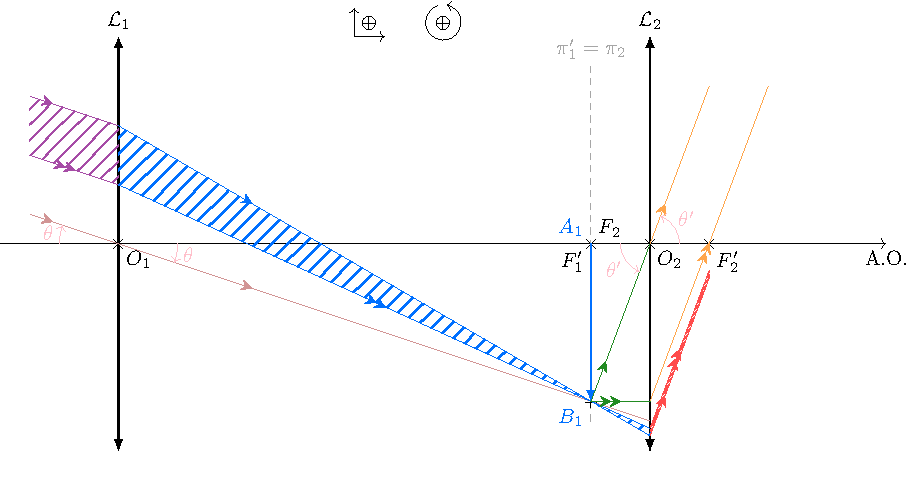
\includegraphics[width=\linewidth]{kepler}
    \captionsetup{justification=centering}
    \caption{Schéma pour la lunette de Kepler.}
    \label{fig:kepler}
\end{figure}

\centering\huge Les angles mal orientés ou dont le signe algébrique ne
correspond pas avec la formule utilisée seront pénalisés.

\end{document}
